\documentclass[14pt,a4paper]{extarticle}
\usepackage[utf8]{inputenc}
\usepackage[T2A]{fontenc}
\usepackage[english,russian]{babel}
%\usepackage{fontspec}
%\setmainfont{Times New Roman} 
\usepackage[unicode]{hyperref}
\usepackage[left=2cm,right=1cm, top=2cm, bottom=2cm]{geometry}
\linespread{1.5}
\usepackage{indentfirst}
\usepackage{amssymb}
\usepackage{cmap}
\usepackage[]{graphicx}
\usepackage{hyperref}
\usepackage{array}
\usepackage{wrapfig}
\usepackage{longtable}
\usepackage{verbatim}
\usepackage{enumitem}
\usepackage{amsmath}
\usepackage{float}
\usepackage{mathtools}
\usepackage{icomma}
\usepackage{caption}
\captionsetup{labelsep=period}
\usepackage{xcolor}
\usepackage{animate}
%\numberwithin{equ`tion}{section}
\newcommand{\ten}[1]{\cdot 10^{#1}}
\hypersetup{
	colorlinks,
	citecolor=black,
	filecolor=black,
	linkcolor=black,
	urlcolor=blue
}

\usepackage{pdfpages}
\newcommand{\whr}{\text{, где}}
\newcommand{\razm}[1]{\hspace{1ex} \ensuremath{\left[\text{#1}\right]}}
\newcommand{\rbf}[1]{\textbf{\ref{#1}}}
\newcommand{\refris}[1]{рис. \rbf{#1}}
\newcommand{\prf}[1]{стр. \textbf{\pageref{#1}}}
\newenvironment{aleq}{\begin{equation}\begin{aligned}}{\end{aligned}\end{equation}}
\renewcommand{\geq}{\geqslant}
\renewcommand{\leq}{\leqslant}
\newcommand{\rt}[1]{_\text{#1}}
\newcommand{\mm}{\razm{мм}}

\renewcommand{\phi}{\varphi}
\renewcommand{\epsilon}{\varepsilon}

\newcommand{\an}[2]{a_{#1}\cos \left({#2}\frac{2\pi x}{P}\right)}
\newcommand{\bn}[2]{b_{#1}\sin \left({#2}\frac{2\pi x}{P}\right)}
\newcommand{\mtrig}[2]{\frac{2}{{#2}\pi}{#1}\left({#2}\frac{2\pi x}{P}\right)}
\author{Максим Зотов}
\title{МТ11-62Б}
\date{Оценка параметров модели скорости травления кремния}
\begin{document}
\maketitle
\tableofcontents
\pagebreak
\selectlanguage{russian}
\renewcommand{\abstractname}{Цель работы}
\begin{abstract}
	Провести оценку физико-химических параметров модели скорости травления кремния
	\begin{center}
		\textbf{Задачи}
	\end{center}
\begin{enumerate}
	\item Принять в качестве исходных данных значения таблицы скорости травления кремния (100)
	при различных температурах
	\item Провести размытие значений таблицы нормально распределенными случайными
	величинами;
	\item Сравнить разные способы оценки параметров модели.
\end{enumerate}
\end{abstract}
\section{Теоретическое обоснование применяемых методов}
Зависимость скорости травления кремния (100) от концентрации реагирующих компонентов
\begin{equation}\label{eq:speed}
	V=k_0\cdot e^{-\frac{E_a}{k_B T}}\cdot C^4_{H_2 O}\cdot C^{\frac{1}{4}}_{KOH}\whr
\end{equation}
\begin{itemize}
	\item $k_0$ -- предэкспоненциальный множитель, характеризующий частоту соударений реагирующих молекул и мало зависящий от температуры
	\item $E_a$ -- энергия активации реакции травления
	\item $k_B$ -- постоянная Больцмана
	\item $T$ -- абсолютная температура
	\item $C^4_{H_2 O}$ -- весовая концентрация воды
	\item $C^{\frac{1}{4}}_{KOH}$ -- весовая концентрация травителя $KOH$ в воде
\end{itemize}
Уравнение Аррениуса имеет вид
\begin{equation}\label{eq:ar1}
	\ln\left(k\left(T\right)\right)=-\frac{E_a}{k_B}\left(\frac{1}{T}\right)+\ln(A)\whr
\end{equation}
\begin{itemize}
	\item $k(T)$ -- константа скорости реакции
	\item $E_a$ -- энергия активации реакции травления
	\item $T$ -- абсолютная температура
	\item $k_B$ -- постоянная Больцмана
	\item $A$ -- предэкспоненциальный множитель, характеризующий частоту соударений реагирующих молекул и мало зависящий от температуры
\end{itemize}

Если пренебречь зависимостью энергии активации $E_a$ и предэкспоненциального множителя $A$ от температуры , то график функции вида
\begin{equation}
	\ln(k(T)) = f \left(\frac{1}{T}\right)
\end{equation}
имеет вид линейной регрессионной зависимости в виде прямой линии. Экспериментальные значения скоростей реакции при различных температурах
могут служить основой для оценки значений $A$ и $E_a$, причем сделать это можно 2
способами.
\subsection{Первый способ оценки}
Представляем выражение \eqref{eq:ar1} в виде регрессионного уравнения вида 
\begin{equation}\label{eq:regress}
	y(x) = ax+b \whr
\end{equation}
\begin{itemize}
	\item $a = -\frac{E_a}{k_B}$ -- тангенс угла наклона прямой к оси абсцисс
	\item $b = \ln(A)$ -- отрезок, отсекаемый прямой \eqref{eq:regress} от оси ординат
\end{itemize}

Из графика эксперементальных значений находят коэффициенты $a$ и $b$, после чего получают значения $A$ и $E_a$
\begin{aleq}\label{eq:EA}
	E_a &= -ak_B\\
	A &= e^b
\end{aleq}

Полученные оценки параметров позволяют рассчитать скорость травления при любой температуре $T$ по уравнению Аррениса
\begin{equation}\label{eq:R}
	R=Ae^{ -\frac{E_a}{k_B T}}
\end{equation}
\subsection{Второй способ оценки}
Выбор координат двух любых точек на построенной прямой и составление системы уравнений с двумя неизвестными $a$ и $b$. 
\begin{aleq}
		\ln\left(R_1\right)=-\EE{1}+\ln(A)\\
		\ln\left(R_2\right)=-\EE{2}+\ln(A)\\
\end{aleq}
Откуда 
\begin{multline}\label{eq:E2}
	\ln(A) = \ln(R_2)+\EE{2} \Rightarrow \ln\left(R_1\right)=-\EE{1} + \ln(R_2)+\EE{2} \Rightarrow \\
	\Rightarrow \ln(R_2)-\ln(R_1)=\EE{1}-\EE{2} \Rightarrow\\ E_a=\frac{k_B(\ln(R_2)-\ln(R_1))}{\ti{1}-\ti{2}}\qquad \qquad \qquad \qquad
\end{multline}
Затем
\begin{equation}\label{eq:A2}
		\ln(A) = \ln(R_2)+\EE{2}\Rightarrow A=e^{\ln(R_2)+\EE{1}}
\end{equation}

Зная энергию активации и константу скорости при какой-либо температуре
\begin{equation}\label{eq:R2}
	\frac{\ln(R_2)}{\ln(R_2)}=\frac{E_a}{k}\left(\ti{1}-\ti{2}\right)\Rightarrow R_2 = R_1 e^{\frac{E_a}{k}\left(\ti{1}-\ti{2}\right)}\whr
\end{equation}
\begin{itemize}
	\item $R_2$ -- скорость, которую необходимо найти
	\item $R_1$ -- известное значение скорости
\end{itemize}
\section{Этапы работы}
\subsection{Вступление}
Рандомизацию чисел можно реализовать несколькими способами. Самый простой из них -- использовать функцию 
\begin{lstlisting}
	RAND();
\end{lstlisting}
которая генерирует нормально распределённую случайную величину от 0 до 1. Эта функция позволяет генерировать случайные числа при нажатии клавиши F9. Поэтому результаты, приведённые в работе и результаты в excel могут несколько отличаться.
\subsection{Таблица исходных данных и её преобразование}
\begin{figure}[H]
	\centering
	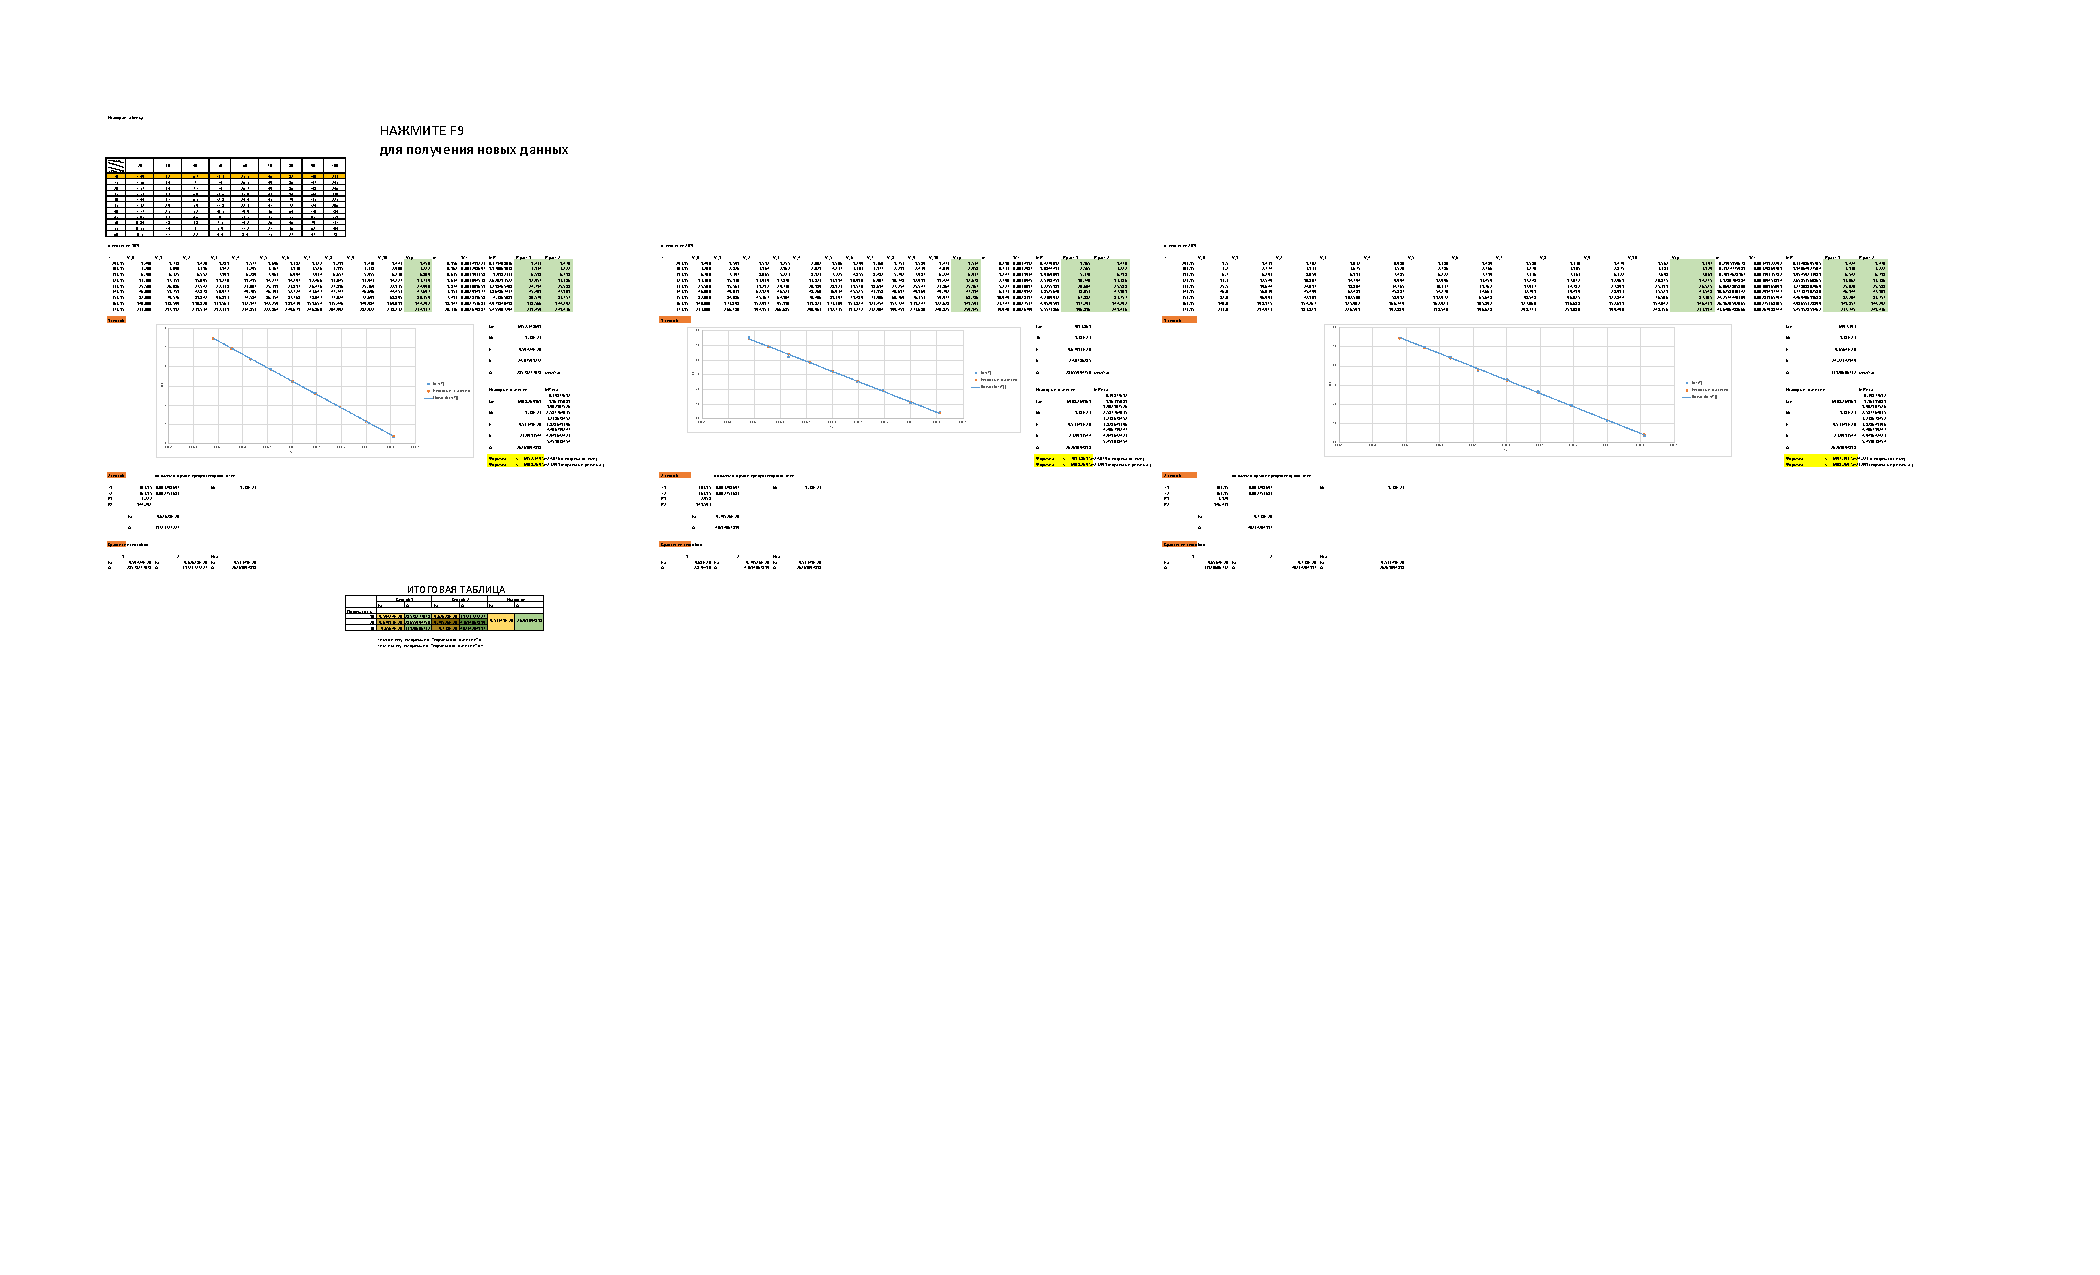
\includegraphics[trim=60 495 840 70, clip, width=0.9\textwidth]{results.pdf}\caption{Таблица исходных параметров процесса травления}\label{fig:ish}
\end{figure}

Производим размытие описанным ранее методом 
\begin{lstlisting}
	V_i = NORM.INV(RAND();$B22;0,1*$B22);
	V_sr = AVERAGE(C22:L22);
	sigma = STDEV.P(C22:M22);
\end{lstlisting}
и получаем следующую таблицу
\begin{figure}[H]
	\centering
	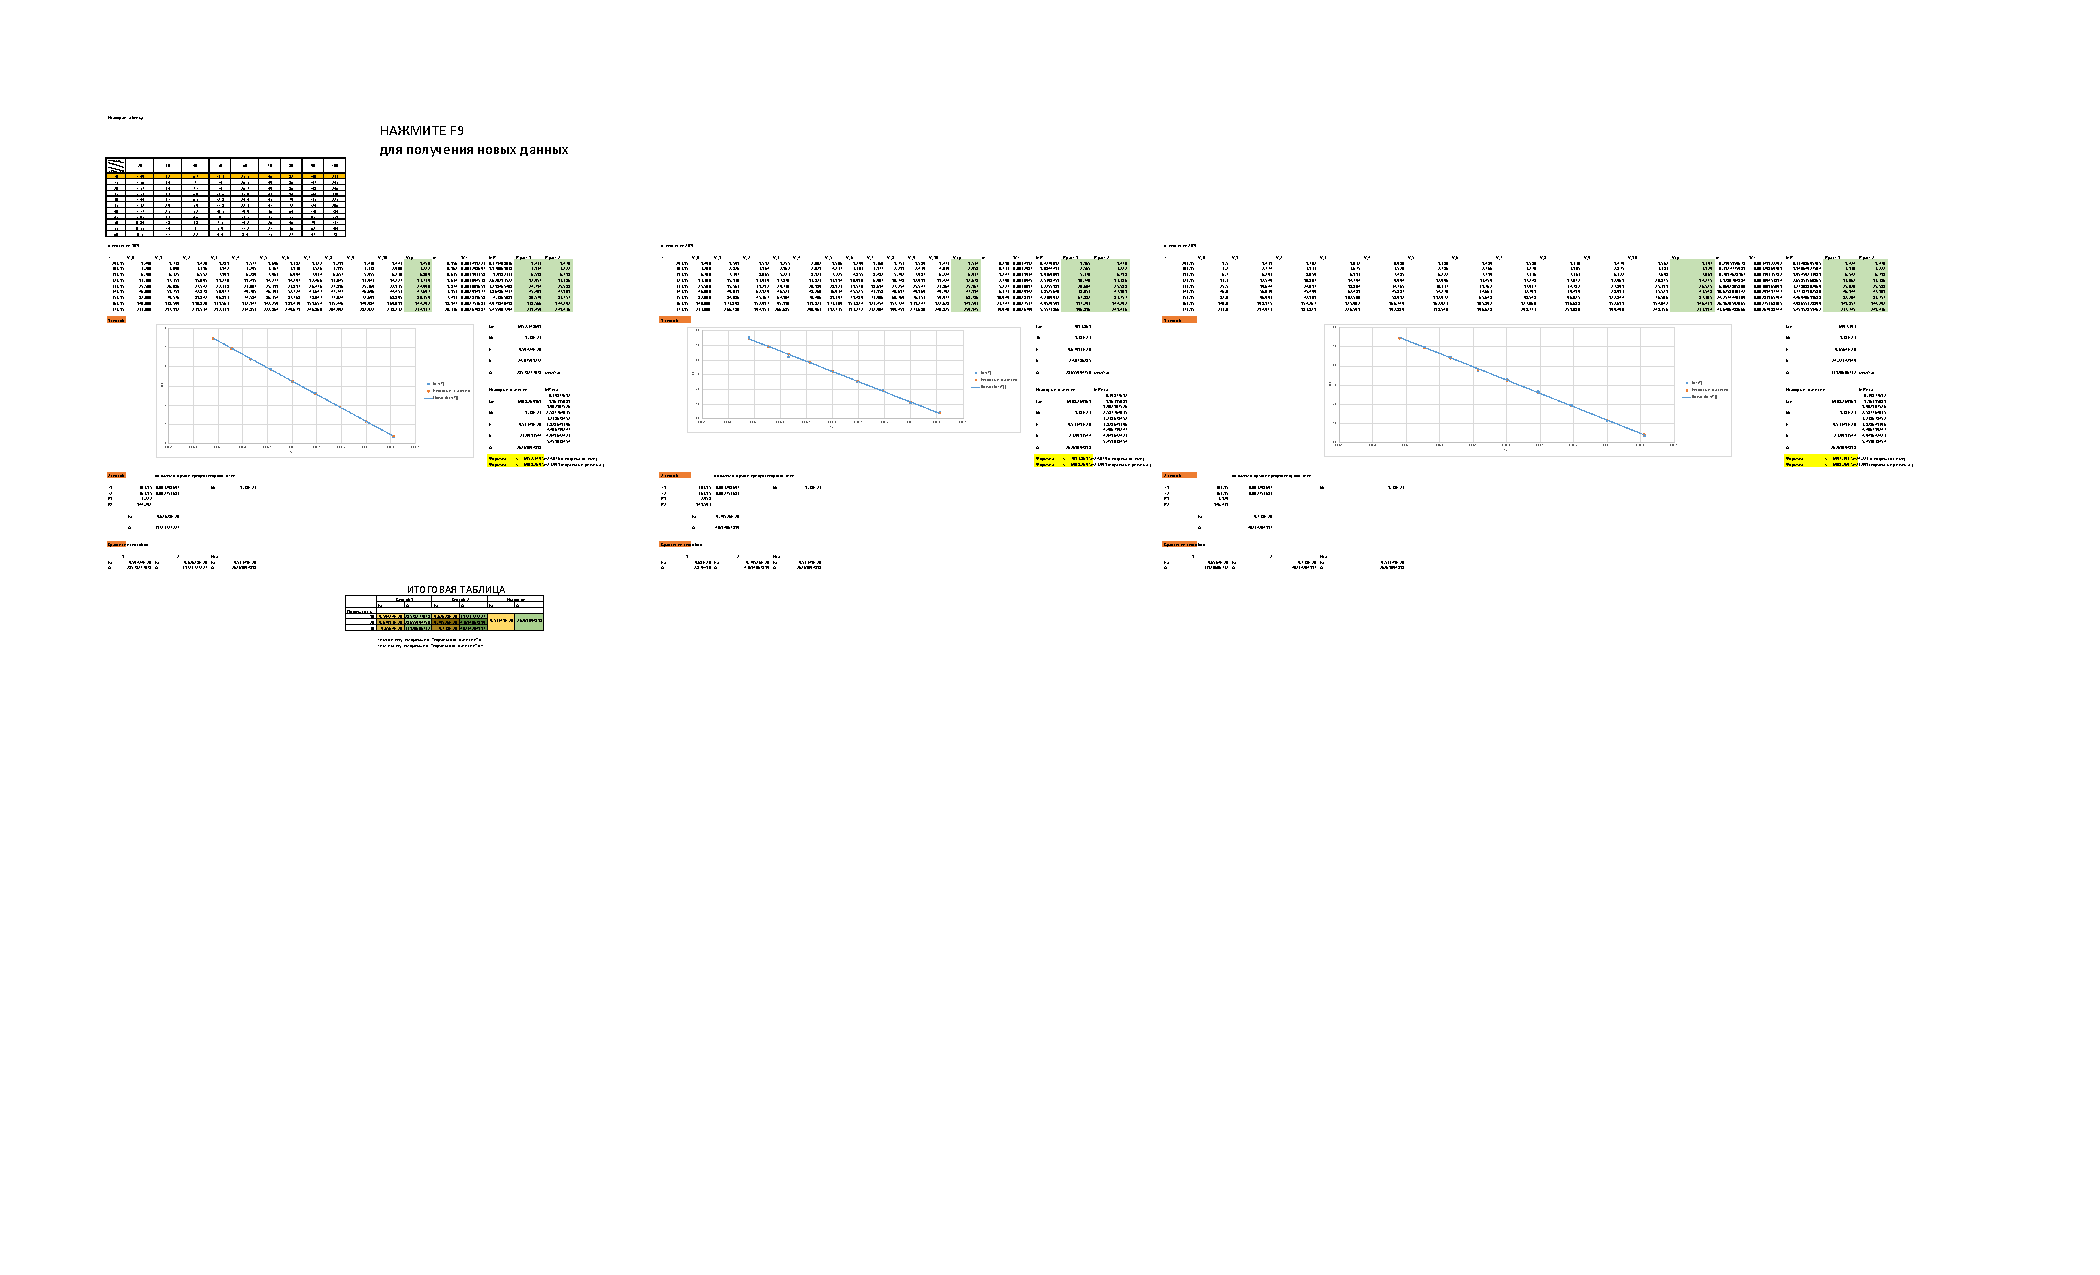
\includegraphics[trim=60 460 762 120, clip, width=0.9\textwidth]{results.pdf}\caption{Таблица эксперементальных значений с отклонением 10\%}\label{fig:razmito10}
\end{figure}
\subsection{Первый способ}
\subsubsection{Построение графика}
Строим график получившихся значений, исходных значений и проводим линию тренда
\begin{figure}[H]
	\centering
	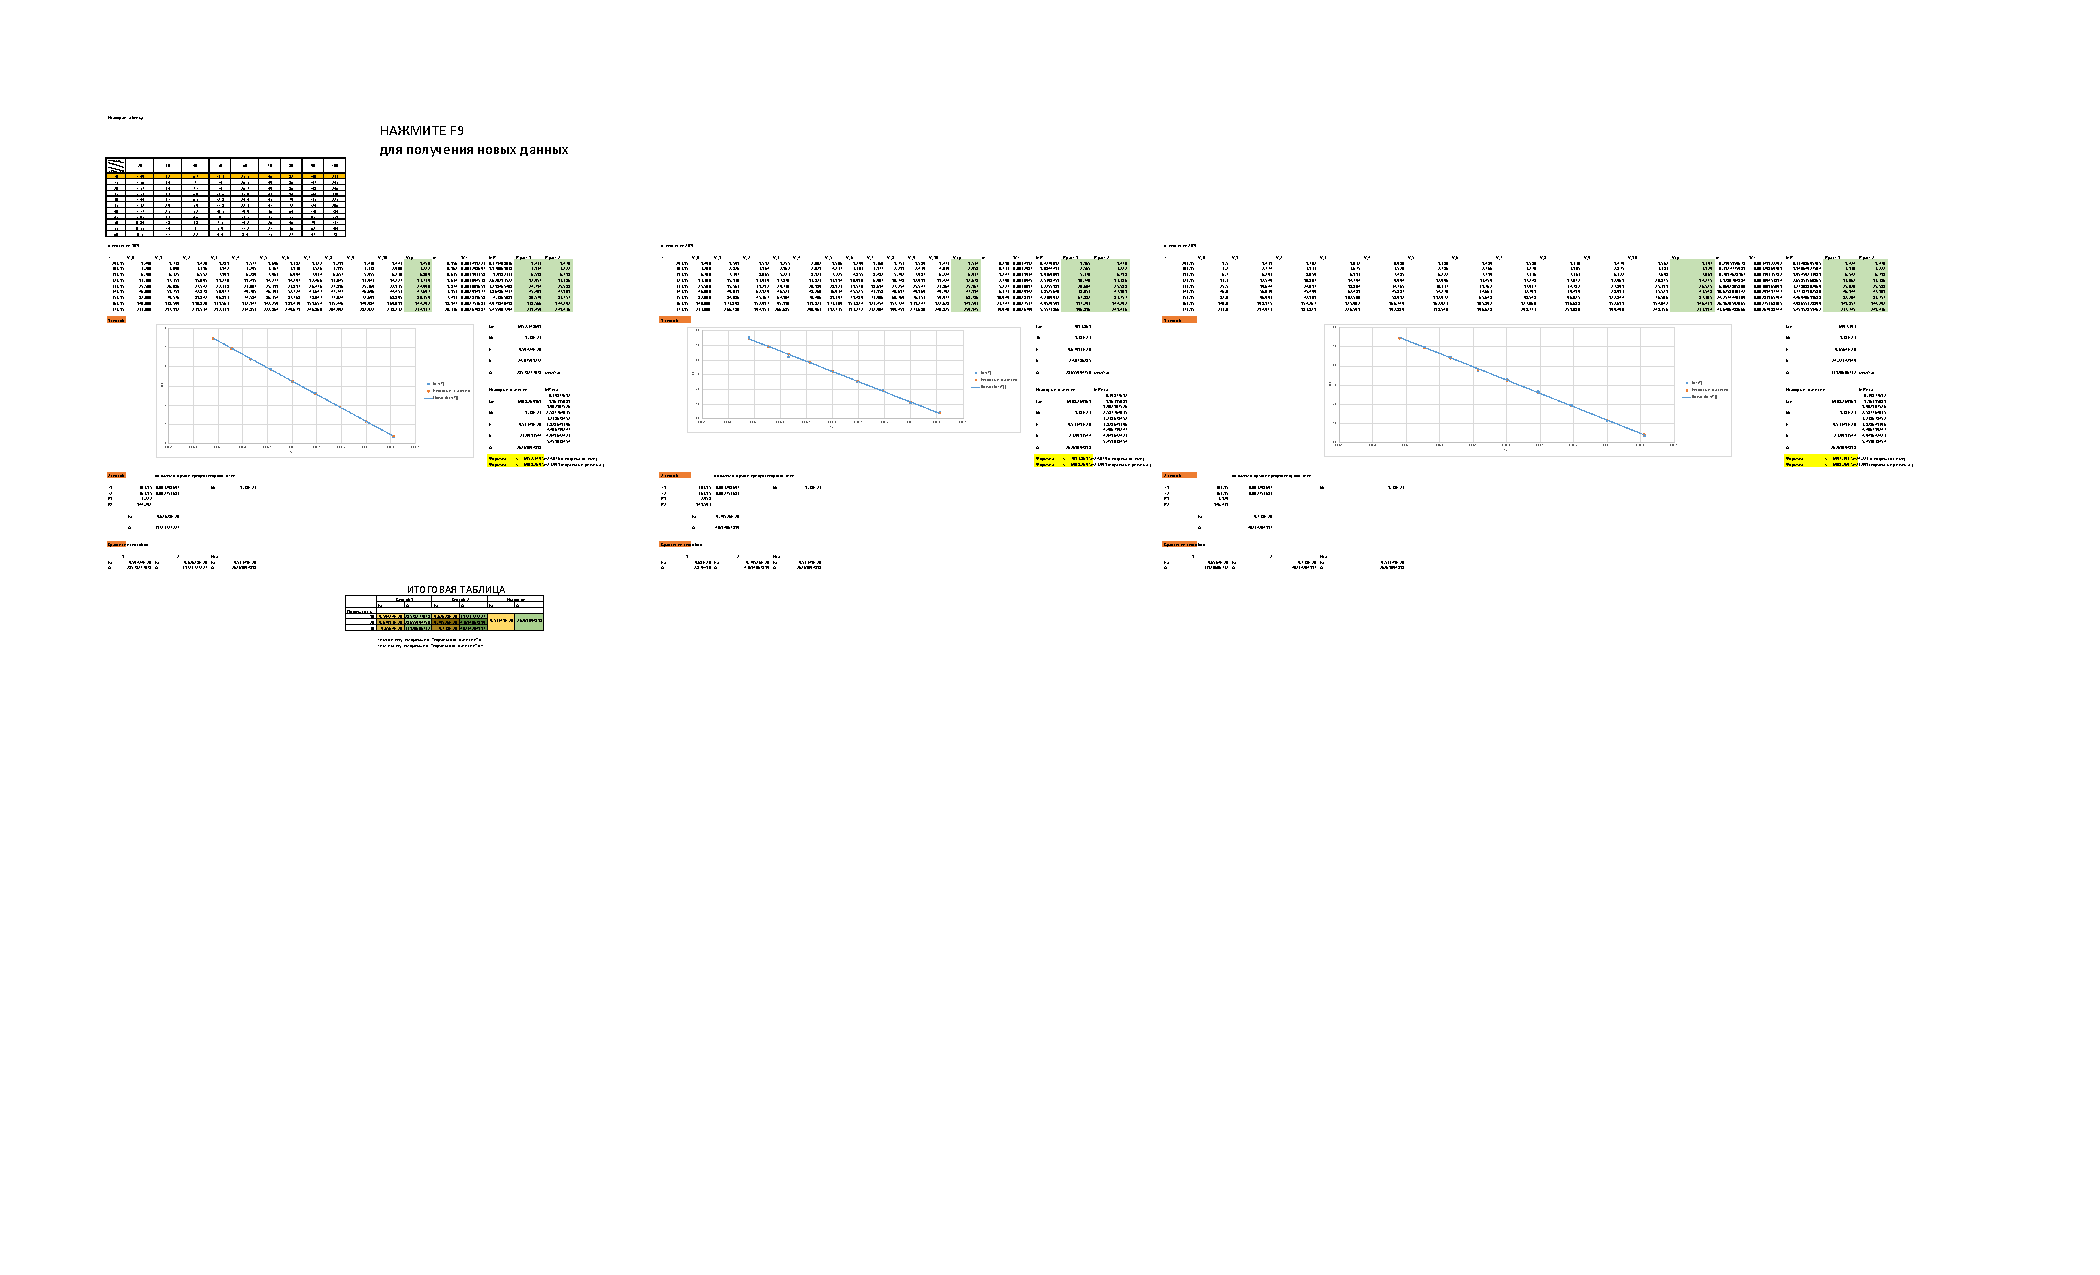
\includegraphics[trim=70 385 716 150, clip, width=\textwidth]{results.pdf}\caption{Полученный график и расчёт коэффициентов}\label{fig:graph10}
\end{figure}

\subsubsection{Вычисление энергии активации и предэкспоненциального множителя}
\begin{enumerate}
	\item \textbf{Энергия активации} из \eqref{eq:EA} представляет из себя отрицательное произведение тангенса угла наклона прямой $a$ на постоянную Больцмана $k_B$
	\begin{lstlisting}
		tan = (P30-P22)/(O30-O22);
		kb = 1,38*10^(-23);
		Ea = -Q33*Q35;
\end{lstlisting}
	\item \textbf{Предэскпоненциальный множитель} $A$ есть ни что иное, как экспонента отрезка, отсекаемого проведённой нами прямой. Поскольку прямая не пересекается с нулём, воспользуемся встроенной в Excel функцией для предсказания её поведения
	\begin{lstlisting}
		b = TREND(LN(B22:B30);O22:O30;0;TRUE());
		A = EXP(Q52);
\end{lstlisting}
\end{enumerate}
\subsubsection{Сравнение полученных уравнений}
Для сравнения экспериментальных и "идеальных" результатов можно привести уравнения двух прямых, вычисленных по формулам
\begin{lstlisting}
	y_pogr10 = CONCATENATE("y = ";ROUND(Q33;3);"*x";"+";ROUND(Q39;3); " (10% error)");
	y_ideal = CONCATENATE("y = ";ROUND(Q46;3);"*x";"+";ROUND(Q52;3); " (ideal result)");
\end{lstlisting}
\begin{figure}[H]
	\centering
	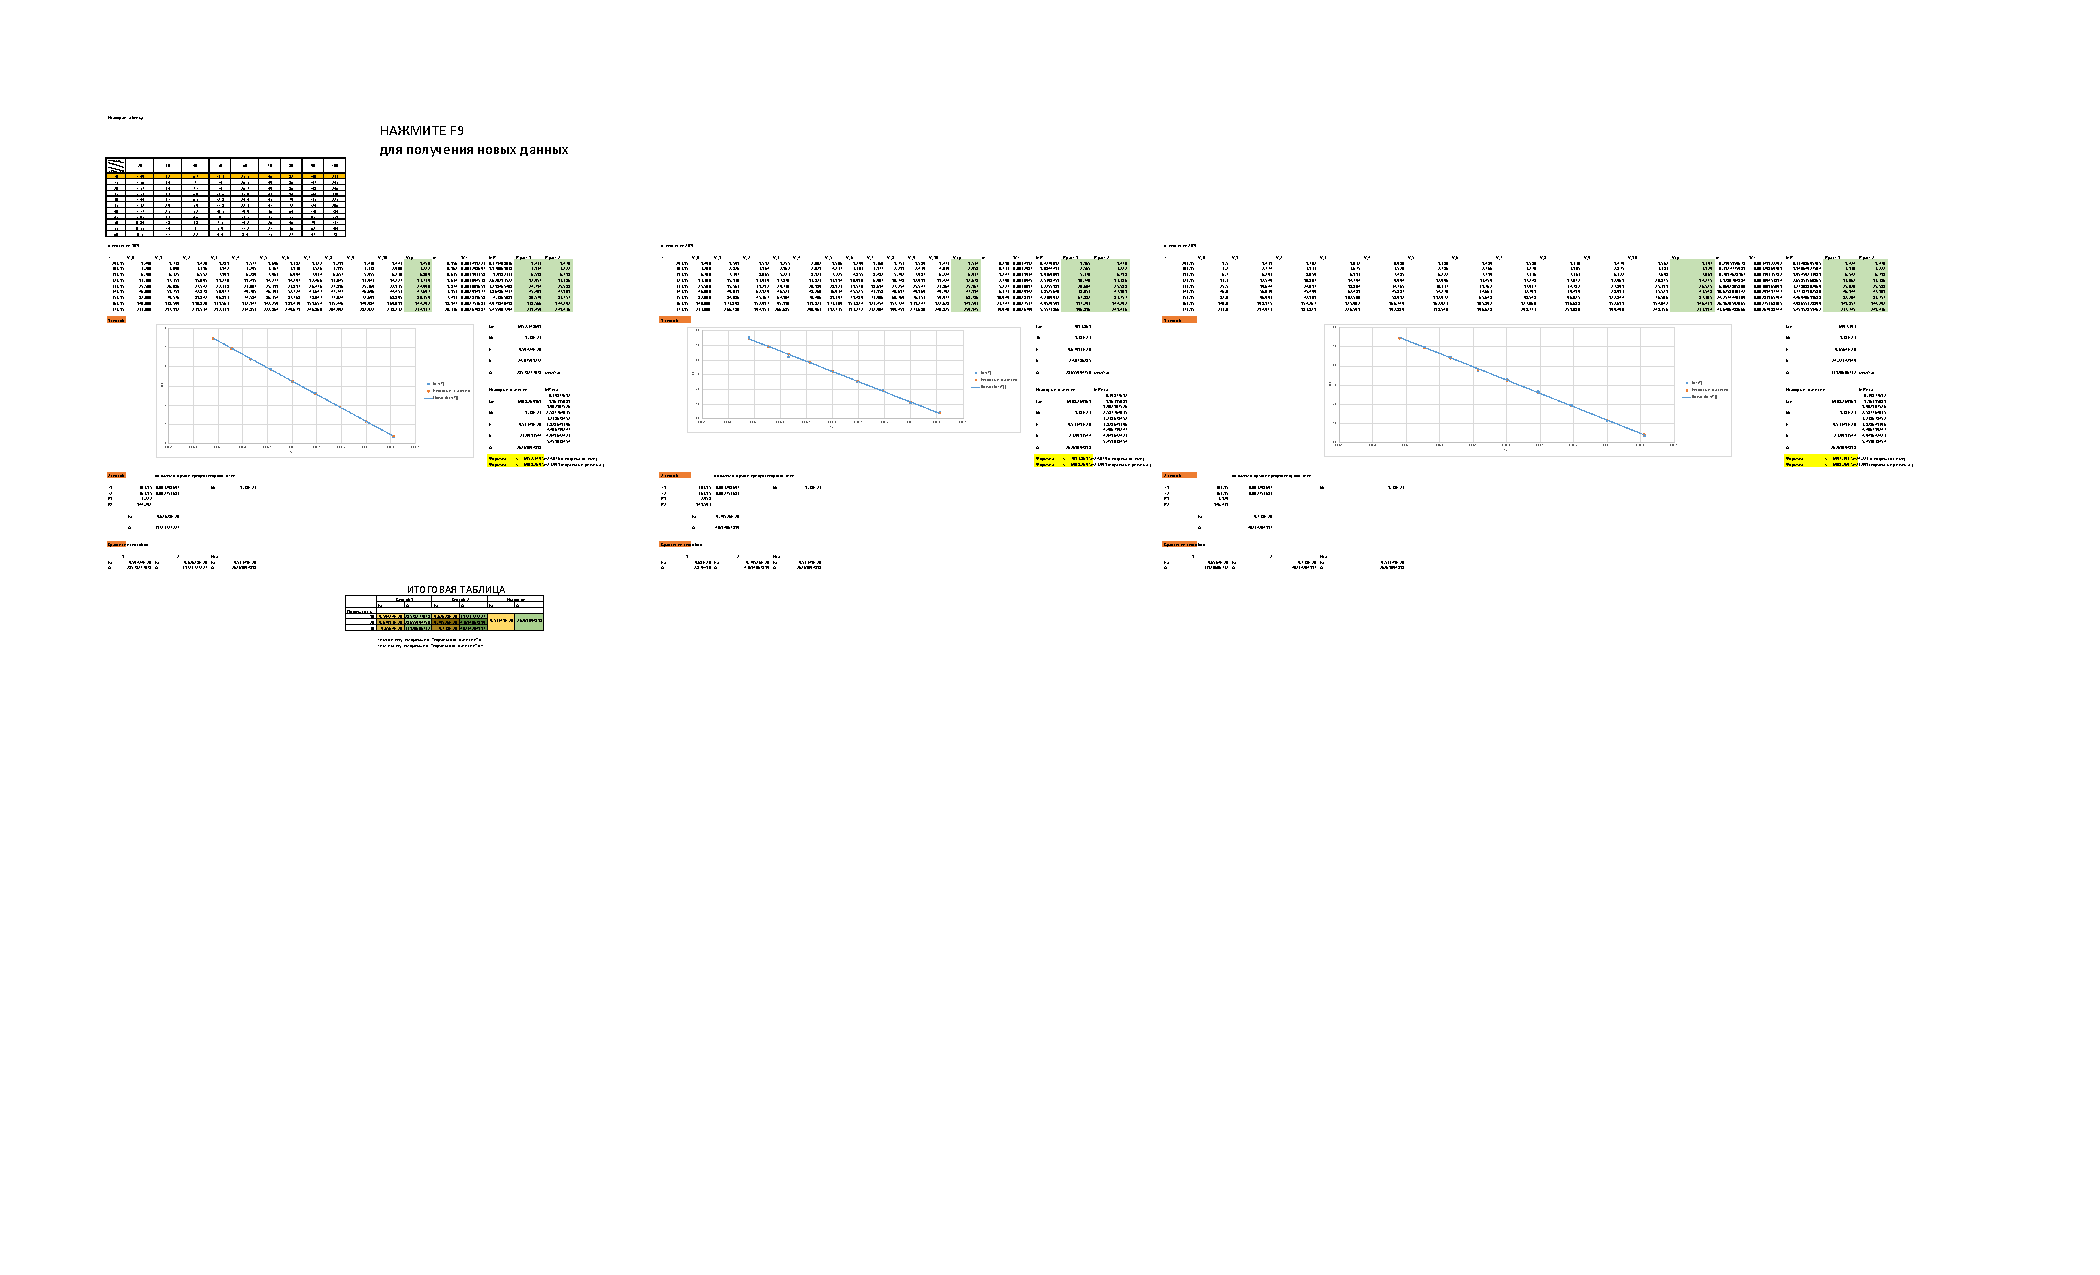
\includegraphics[trim=230 385 716 217, clip, width=\textwidth]{results.pdf}\caption{Полученные уравнения}\label{fig:uravn}
\end{figure}
\subsection{Второй способ}
\subsubsection{Выбор расчётных точек}
Выбираем на графике 2 точки (выберем вторую и предпоследнюю, чтобы исключить "краевые" эффекты)
\begin{lstlisting}
	T1 = A23; R1 = M23;
	T2 = A29; R2 = M29;
\end{lstlisting}
\subsubsection{Вычисление энергии активации и предэкспоненциального множителя}
Из полученных в \eqref{eq:E2} и \eqref{eq:A2} получаем
\begin{lstlisting}
	E_a = (LN(B64)-LN(B63))*F61/(C61-C62);
	A = EXP(LN(B63)+C66*C61/F61);
\end{lstlisting}
\begin{figure}[H]
	\centering
	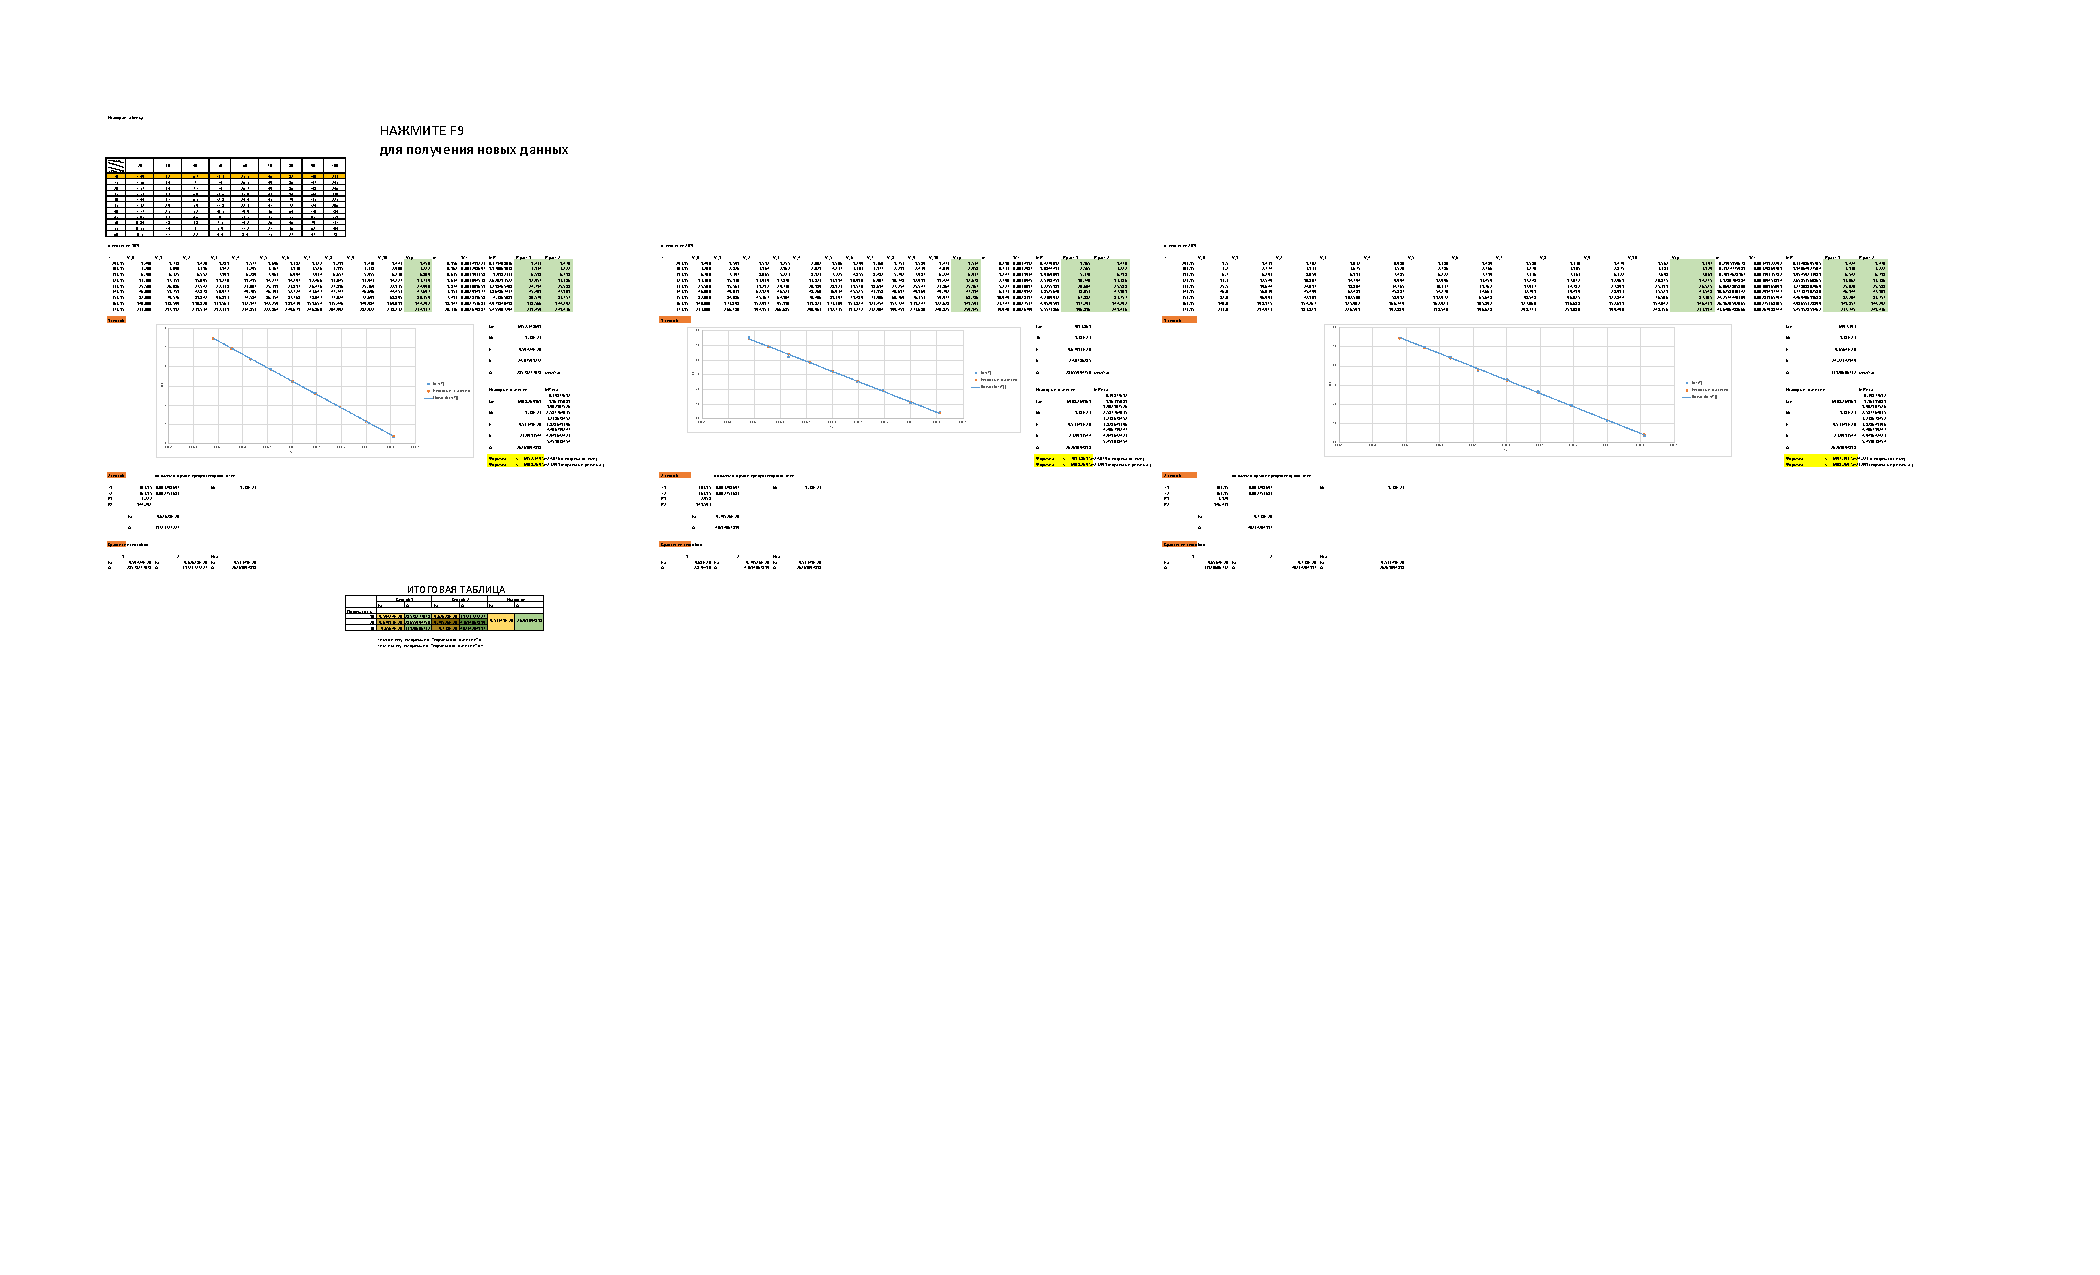
\includegraphics[trim=50 355 880 222, clip, width=0.5\textwidth]{results.pdf}\caption{Данные для расчёта по второму способу}\label{fig:sposob2}
\end{figure}
\subsection{Вычисление скоростей реакции по моделям}
Полученные модели позволяют получить скорости реакции при известных энергии активации и предэкспоненциальном множителе
\begin{aleq}
	R\rt{расч 1} (T)&= Ae^{\EE{}}\\
	R\rt{расч 2} (T) &= R_0 e^{\EE{0}} \text{\hspace{3mm}, где $R_0, T_0$ -- известные значения }
\end{aleq}
В Excel расчёт выглядит следующим образом
\begin{lstlisting}
	R_1 = Q$41*EXP(-Q$37*O22/Q$35);
	R_2 = $M$23*EXP($C$66/$F$61*($O$23-O22));
\end{lstlisting}
\begin{figure}[H]
	\centering
	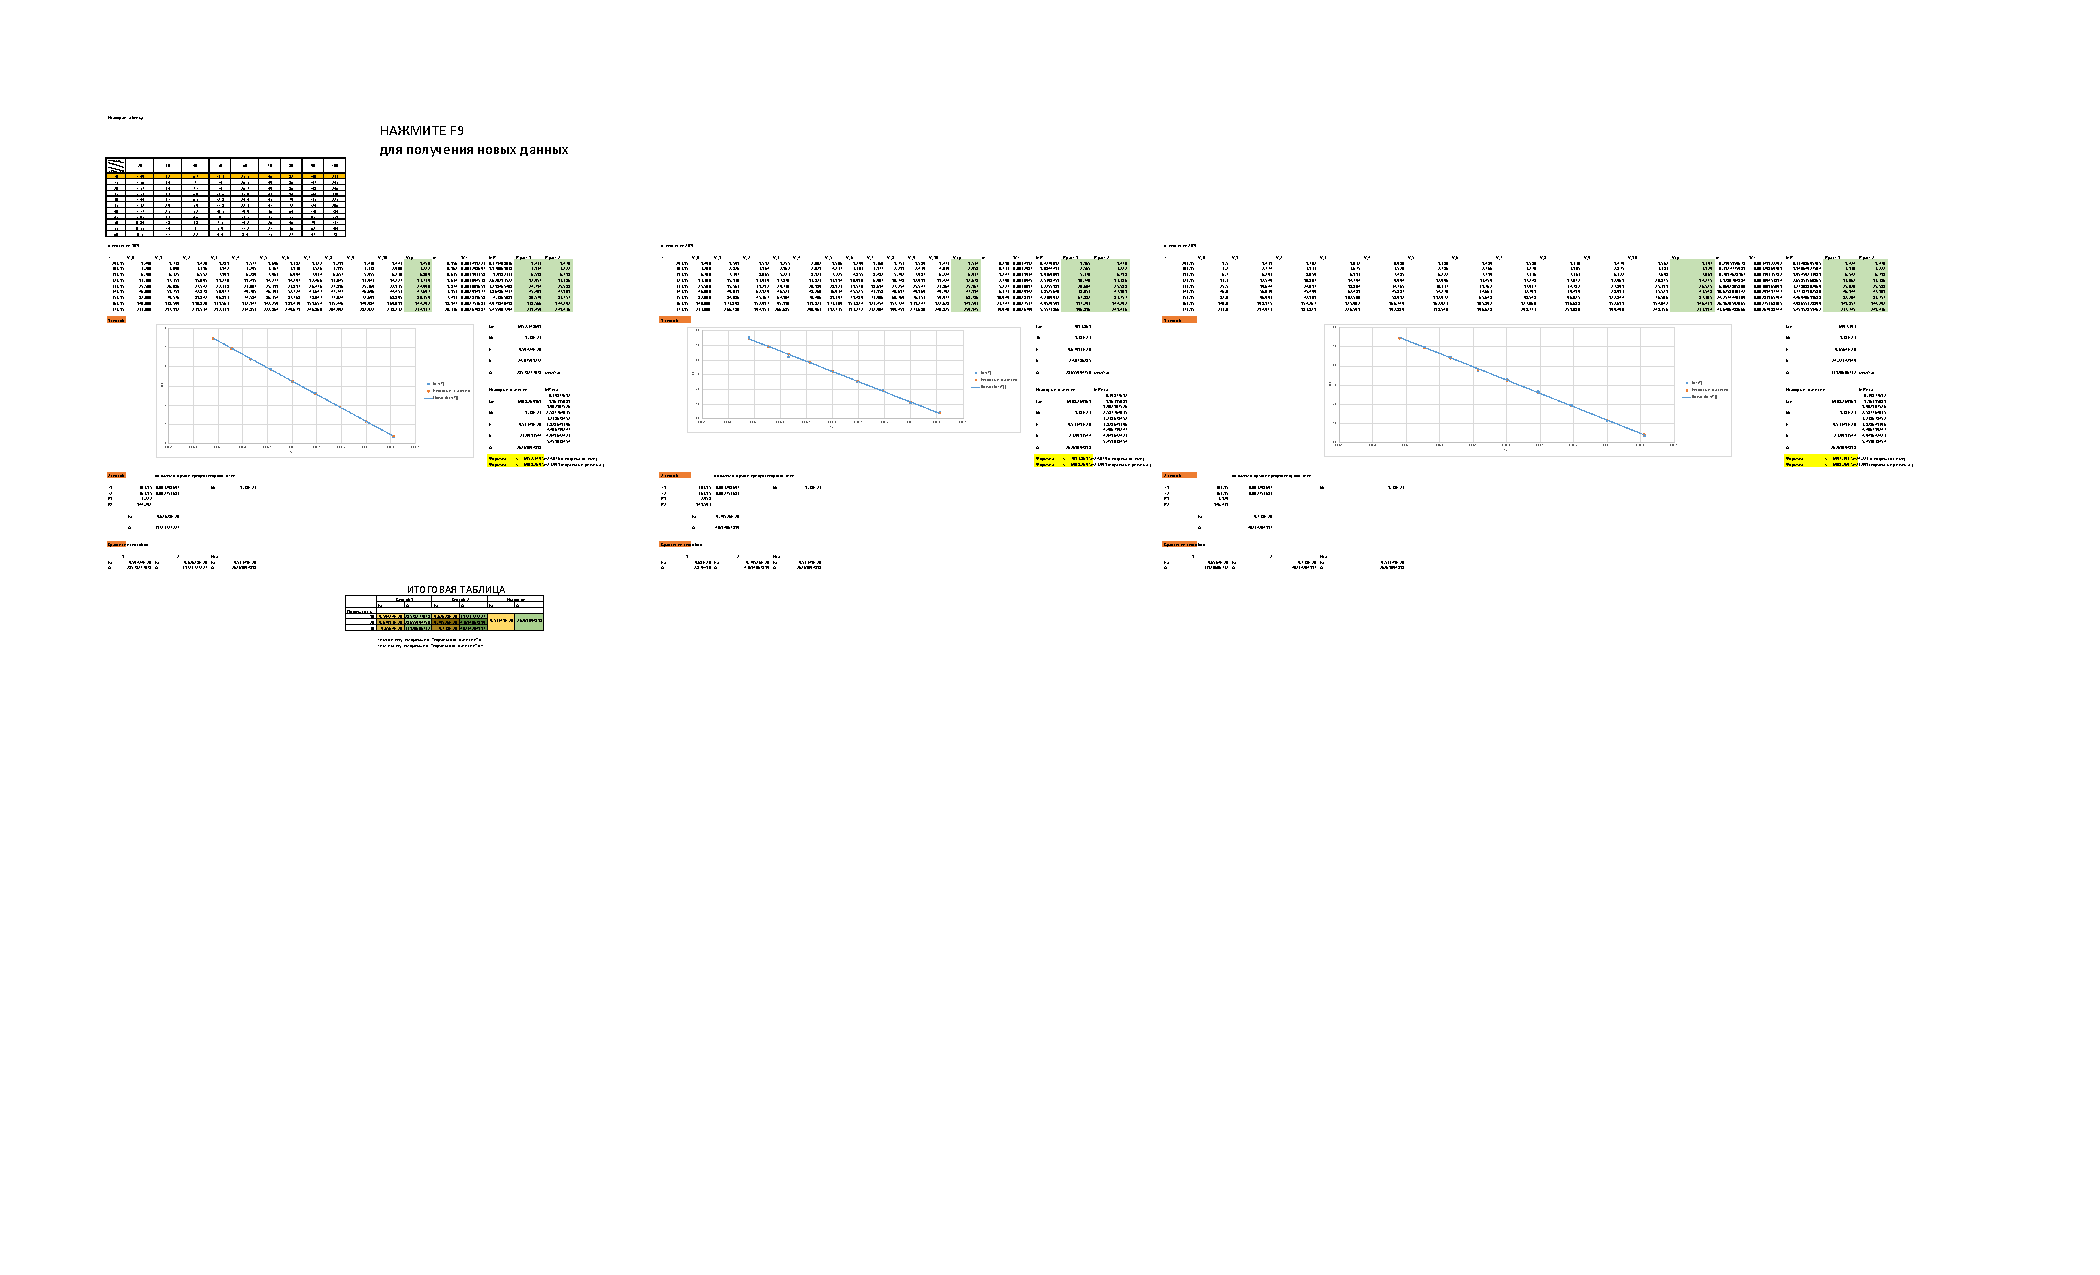
\includegraphics[trim=194 460 733 120, clip, width=0.6\textwidth]{results.pdf}\caption{Получившиеся значения скоростей двумя способами}\label{fig:res10}
\end{figure}
\section{Итоги}
\subsection{Таблица результатов}
После проведения аналогичных опытов для погрешностей 20\% и 30\% получим итоговую таблицу
\begin{figure}[H]
	\centering
	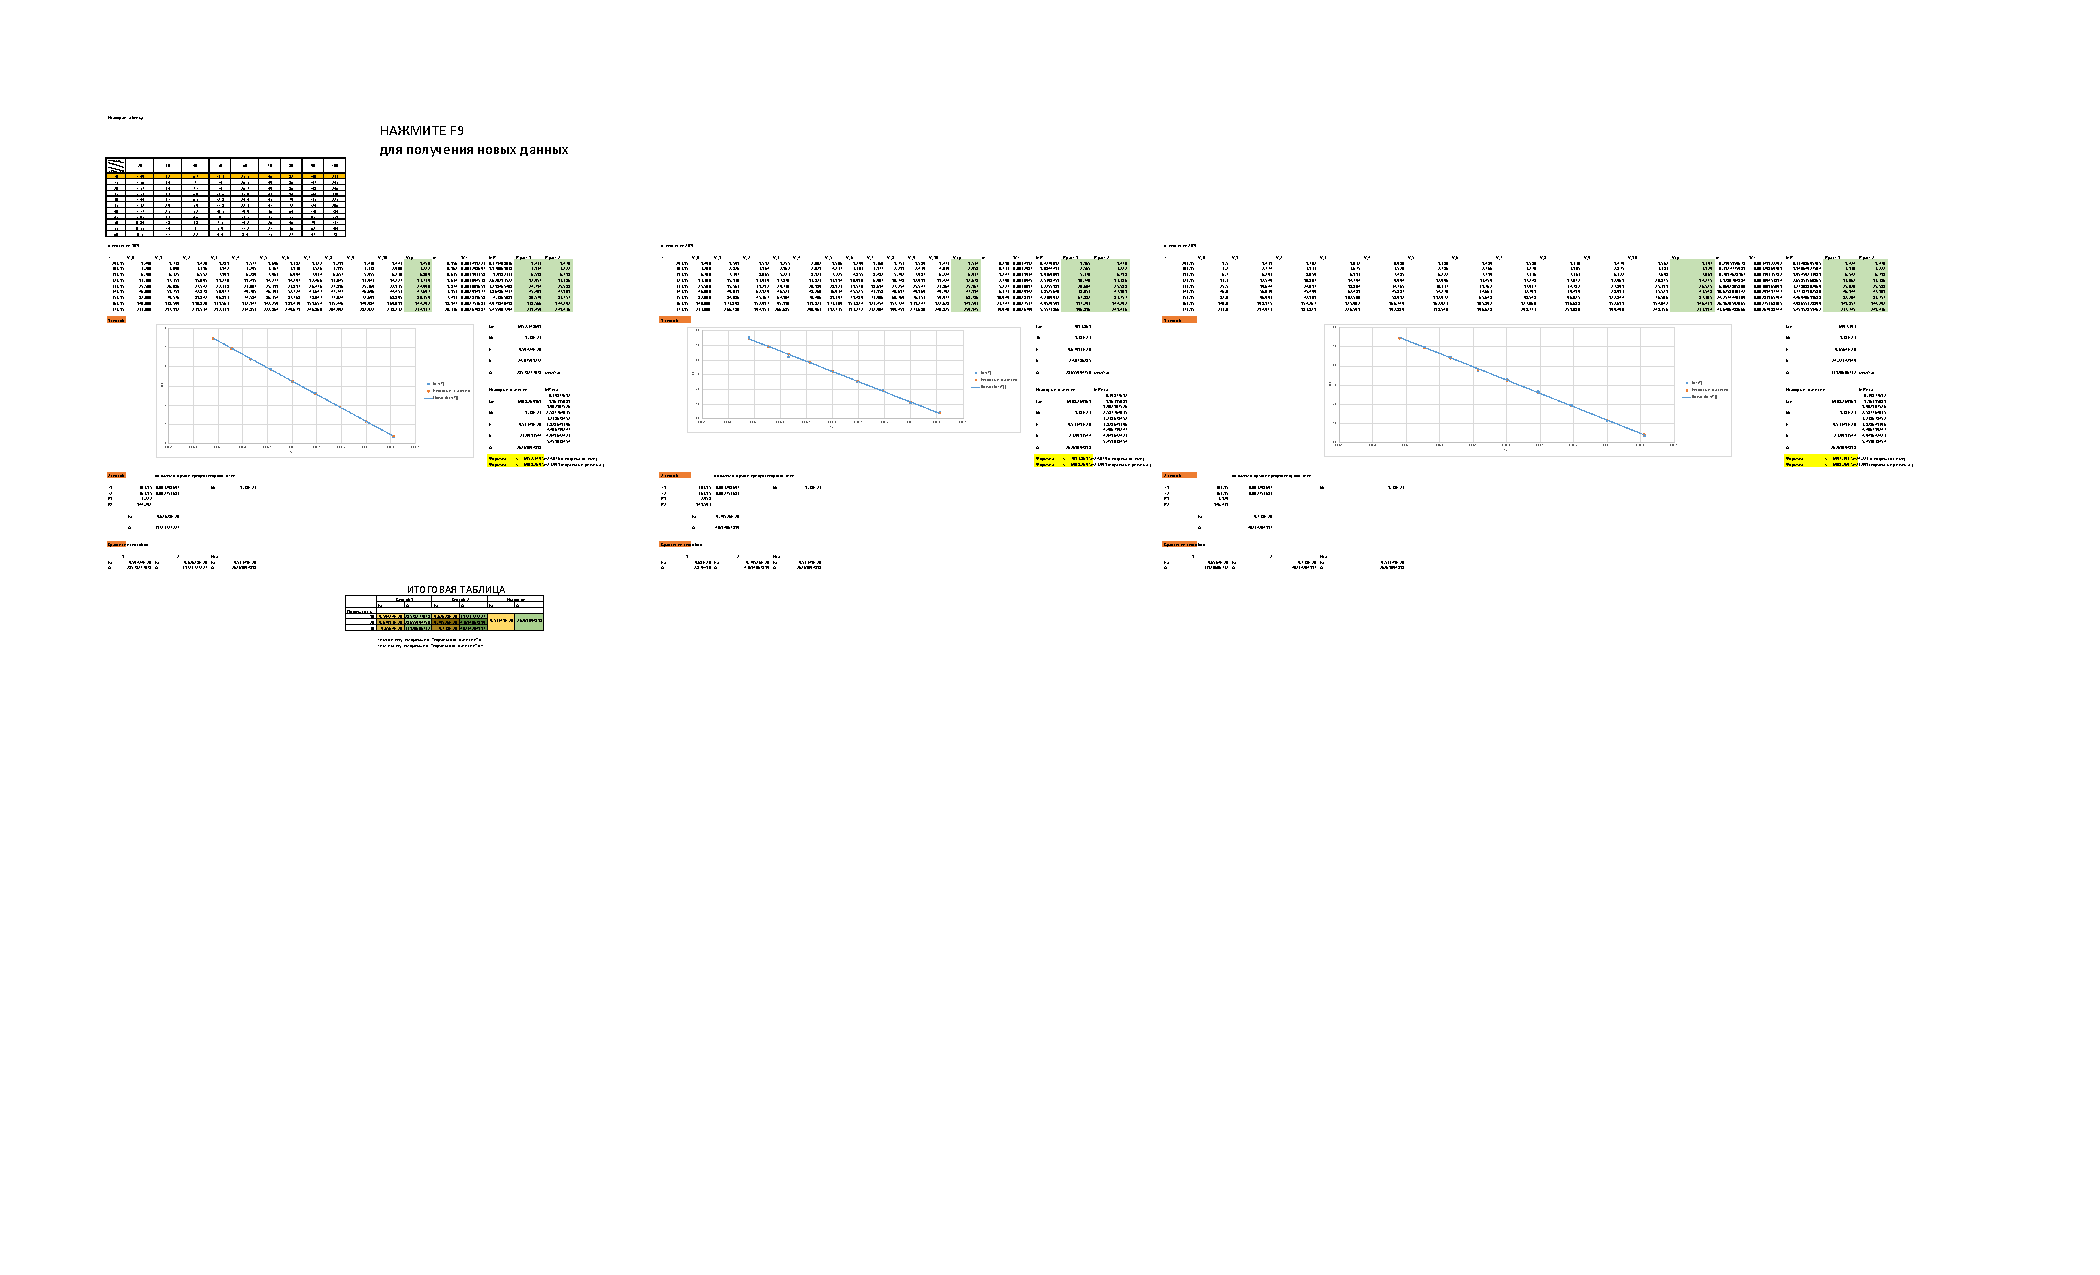
\includegraphics[trim=160 300 740 280, clip, width=0.9\textwidth]{results.pdf}\caption{Таблица результатов}\label{fig:tabl}
\end{figure}
\subsection{Вариация таблицы результатов}
На рис. \rbf{difference} показана серия результатов моделирования
\begin{figure}[H]
	\centering
	\animategraphics[trim=120 100 140 230 ,loop,controls={play,step},width=0.8\textwidth]{24}{animate/Screenshot_}{1}{100}
	\caption{Вариация результатов при изменении значений скорости}\label{difference}
\end{figure}
\subsection{Вывод}
Случайные погрешности могут оказывать значительное влияние на результаты эксперимента. Можно заметить, что иногда результаты первого метода получаются более точными, чем результаты второго и наоборот. В среднем первый метод оказывается точнее второго. 

Необходимо минимизировать погрешности во избежание сильного расхождения результатов.
\end{document}